The previous chapter on motion planning and control introduced techniques for developing mathematical models to describe robot motion by analyzing its kinematics and dynamics. These models are typically expressed in the form of differential equations that are functions of a set of generalized coordinates/velocities and inputs to the system.
The next step is to discover how these models can be leveraged for robot motion planning and control. In particular this chapter and the next will focus on robot control, where the goal is to determine what inputs to apply to the system to achieve desirable behavior. To address the robot control problem a \textit{control law} must be developed, which is a set of rules or a mathematical function that determines what inputs should be applied to the system at any given time.

The ecosystem of techniques for robot control is vast, and control laws can generally be categorized in several ways. One of the most fundamental classifications for a control law is if it is \textit{open-loop} or \textit{closed-loop}. Open-loop control laws do not rely on observations to influence the choice of control input, while closed-loop control laws do. As a practical example, suppose you are standing in a room and wanted to walk to the other side and sit in a chair. For open-loop control you might look at where the chair is relative to your current position, think about how to walk there, and then \textit{with your eyes closed} walk to the chair and sit. Alternatively, for closed-loop control you might keep \textit{your eyes open} the whole time.

In practice, open-loop control laws suffer from robustness issues since they do not make corrections based on real-time observations. However, open-loop control is still an extremely important topic within the context of robotics.
In particular, suppose you are interested not just in getting your robot from one point to another, but doing so in the \textit{best} or \textit{optimal} way. This problem, known as \textit{trajectory optimization} or \textit{optimal control}\footnote{The terms trajectory optimization and optimal control will often be used interchangeably.}, can be solved to obtain an optimal trajectory for the robot along with the corresponding sequence of control inputs. In theory, applying this optimal control sequence as an open-loop control law would then make the robot follow the optimal trajectory. 

This chapter will discuss several common techniques related to optimal control and trajectory optimization, including a brief review on dynamic/kinematic models, the formulation of the optimal control problem, approaches for solving optimal control problems, and some other topics useful in the context of robotics. The next chapter will then focus on the development of closed-loop control laws, including approaches that leverage the open-loop optimal control techniques discussed here.

\notessection{Open-Loop Motion Planning \& Control}
This chapter and the next will focus on two of the most fundamental classifications for a control law, namely whether it is \textit{open-loop} or \textit{closed-loop}. In particular, this chapter will focus on open-loop control laws that arise from the study of optimal control and trajectory optimization problems\cite{Kirk2004}\cite[\baselineskip]{Murray2009}. In general, open-loop control laws depend only on time and initial condition of the system.

\begin{definition} [Open-loop control] \label{def:openloop}
If the control law is determined as a function of time for a specified initial state value, i.e., 
\begin{equation}
    \bm{u}(t) = f ( \x ( t_0 ) , t ),
\end{equation}
then it is said to be in open-loop form.
\end{definition}


\subsection{Kinematic and Dynamic Models}
Chapter 1 discussed techniques for deriving kinematic and dynamic models of a robot in the form of ordinary differential equations (ODE). Such models are extremely useful in the context of robot motion planning and control, and are essential in the context of optimal control.
For the remainder of this chapter it will be assumed that such a model has already been identified and is expressed in the form
\begin{equation} \label{eq:dynamics}
    \dot{\x}(t) = a(\x(t),\bm{u}(t),t),
\end{equation}
where $\x \in \R^n$ may be comprised of generalized coordinates $\xi$ and velocities $\dot{\xi}$ and will be referred to as the robot's \textit{state}, $\bm{u} \in \R^m$ is the control input, and the function $a : \R^n \times \R^m \times \R \xrightarrow{} \R^n$ defines the model. While the set of ODEs \eqref{eq:dynamics} may have been derived by considering kinematics, dynamics, or a combination of the two, this model will be generally referred to as the robot's \textit{dynamics} model.

For clarity, note that \eqref{eq:dynamics} is a compact expression written in vector form for the system of $n$ first-order differential equations 
\begin{align*}
    \dot{x}_1(t)&=a_1(x_1(t), x_2(t), \dots, x_n(t), u_1(t), u_2(t), \dots, u_m(t), t)\\
    \dot{x}_2(t)&=a_2(x_1(t), x_2(t), \dots, x_n(t), u_1(t), u_2(t), \dots, u_m(t), t)\\
&\vdots \\
    \dot{x}_n(t)&=a_1(x_1(t), x_2(t), \dots, x_n(t), u_1(t), u_2(t), \dots, u_m(t), t),
\end{align*}
where $x_i$ is the $i$-th component of the vector $\x$ and $u_j$ is the $j$-th component of the vector $\bm{u}$.

Solutions to the set of differential equations \eqref{eq:dynamics} are trajectories of the system. Given an initial condition $\x(t_0)$ and a control function $\bm{u}(t)$ defined for $t \geq t_0$, any technique for solving ODEs can be applied to compute the state trajectory $\x(t)$ for $t > t_0$. Common numerical integration approaches for solving the ODE system include the Runge-Kutta schemes, of which the most common are the forward or backward Euler schemes. The forward Euler scheme approximates $\dot{\x}(t) \approx \frac{\x_{i+1} - \x_i}{h_i}$ with $h_i = t_{i+1} - t_{i}$ and evaluates $a$ at time $t_i$. This leads to the recursive update
\begin{equation}
\x_{i+1} = \x_{i} + h_i a(\x_i,\bm{u}_i,t_i), \quad i = 0, 1,\dots
\end{equation}
where $\bm{u}_i = \bm{u}(t_i)$ and $\x_i = \x(t_i)$.


\subsection{Optimal Control Problem}
Perhaps the most common open-loop control laws used for motion planning and control in robotics are synthesized by formulating and solving optimal control problems. These problems are designed to answer the question: from the current state of the robot, $\x(t_0)$, what future control inputs $\bm{u}(t)$ would make the robot follow an optimal future trajectory? In general, generating optimal open-loop control laws require three major components:
\begin{enumerate}
    \item A model \eqref{eq:dynamics} that describes the robot's motion as a function of the input, developed by analyzing the robot's kinematics/dynamics.
    \item A metric that defines the quality of a particular trajectory, known as a \textit{cost function} or a \textit{reward function}\footnote{The term \textit{cost} is more commonly used in optimal control literature, while \textit{reward} is used in the reinforcement learning literature.}.
    \item An algorithm for searching the space of possible control inputs to find one that corresponds to an optimal trajectory\footnote[][\baselineskip]{For example, convex optimization solvers}.
\end{enumerate}


\subsubsection{Problem Formulation}
In this chapter the performance metric that defines the quality of a particular trajectory will be referred to as the \textit{cost function}. The standard form for defining the cost function in optimal control problems is
\begin{equation} \label{eq:cost}
J(\x(t), \bm{u}(t), t) = h(\x(t_f),t_f) + \int_{t_0}^{t_f} g(\x(t),\bm{u}(t),t) dt.
\end{equation}
where $h(\x(t_f),t_f)$ is referred to as a \textit{terminal cost} and where the integral can be viewed as a sum of \textit{stage costs} induced along the path from times $t_0$ to $t_f$.
In robotics, the function $J$ might quantify objectives such as ``get from point A to point B as quickly as possible” or “get from point A to point B while using as little effort as possible”. 

Constraints can also be considered in the optimal control problem. In the field of robotics it is common to consider constraints on the state and control that are expressed compactly as
\begin{equation} \label{eq:constraints}
\x(t) \in \mathcal{X}, \quad \bm{u}(t) \in \mathcal{U},
\end{equation}
where $\mathcal{X}$ is the set of all \textit{admissible} states and $\mathcal{U}$ is the set of all \textit{admissible} control inputs. A common way to define the sets $\mathcal{X}$ and $\mathcal{U}$ is by a set of inequalities on $x$ and $u$, respectively. For example, let's assume the first element of $\x$ is constrained by $x_1 \geq 0$, then $\mathcal{X} = \{x \:|\: x_1 \geq 0\}$ such that any vector $\x$ with $x_1 \geq 0$ belongs to the set $\mathcal{X}$ (and is therefore \textit{admissible}). \marginnote{Constraints are commonly used in the context of robotics to account for actuator limits (e.g. how fast the wheels can turn, how much torque a motor can produce), or constraints on the trajectory itself (e.g. avoid collisions with surrounding objects).}

The optimal control problem is then expressed as an optimization problem over the state trajectory $\x(t)$ and control inputs $\bm{u}(t)$ with the goal of minimizing the cost function \eqref{eq:cost} while also satisfying the constraints \eqref{eq:constraints}.

\begin{definition}[Optimal Control Problem] 
An optimal control problem seeks an \textit{admissible control} $\bm{u}(t)$ which causes the system (\ref{eq:dynamics}) to follow an \textit{admissible trajectory} $\bm{x}(t)$ that minimizes a performance metric $J(\x(t),\bm{u}(t),t)$. This problem can be expressed as an optimization problem:
\begin{equation} \label{eq:OCP}
\begin{split}
\underset{\bm{u},\x}{\text{minimize}} \:\: & h(\x(t_f),t_f) + \int_{t_0}^{t_f} g(\x(t),\bm{u}(t),t) dt,\\
\text{s.t.} \:\:& \dot{\x}(t) = a(\x(t),\bm{u}(t),t), \\
&\x(t) \in \mathcal{X}, \quad \bm{u}(t) \in \mathcal{U}, \\
&\x(t_0) = \x_0,
\end{split}
\end{equation}
where $t_0$ is the initial time, $t_f$ is either a fixed final time or an optimization variable, and $x_0$ is a known initial condition.
\end{definition} 

The solution to the optimal control problem \eqref{eq:OCP} is an admissible and optimal trajectory defined over the interval $t \in [t_0, t_f]$, and is denoted by $\bm{u}^*(t)$ and $\x^*(t)$.

\subsubsection{Solving the Optimal Control Problem}
Once the optimal control problem \eqref{eq:OCP} has been formulated, the next step is to find a solution. However, this can be challenging since \eqref{eq:OCP} is an infinite-dimensional optimization problem (because the optimization is over an infinite-dimensional function and not a finite set of parameters). Unless an analytical solution to the problem can be found, this problem must be transformed into a finite dimensional problem so that it can be solved numerically on a computer.
In general, algorithms for numerically solving optimal control problems can be classified as either \textit{direct} or \textit{indirect} methods. 

\paragraph{Direct Methods:}
Direct methods follow a ``first discretize, then optimize" approach. In the first step the problem \eqref{eq:OCP} is converted into a finite-dimensional problem by discretizing the functions $\x(t)$ and $\bm{u}(t)$. For example this might be accomplished by defining the new optimization variables to be $\x(t_i)$ and $\bm{u}(t_i)$ for a finite number of time points $t_i$. This finite-dimensional optimization problem is generally referred to as a \textit{nonlinear program} (NLP), which can be solved with existing numerical algorithms\footnote{Several solvers for solving general NLPs include IPOPT and SNOPT, and software packages for solving optimal control problems using the direct method include DIDO, PROPT, and GPOPS.}.

\paragraph{Indirect Methods:}
Indirect methods follow a ``first optimize, then discretize" approach. These methods first derive the necessary conditions of optimality, which are expressed as a two-point boundary value problem. This two-point boundary value problem is essentially a set of ODEs with boundary conditions at two points\footnote{This is in contrast to initial value problems, which have a single boundary condition and can easily be numerical integrated to find a solution.} that must be numerically solved.

\vspace{\baselineskip}
Indirect methods are less commonly used in robotics because the derivation of the necessary conditions of optimality must be done on a case by case basis, and can become quite challenging. They become particularly difficult to use when constraints are imposed in the problem. In contrast, direct methods offer much more flexibility and have been quite successful in practice.

\subsection{Differential Flatness}
Solving optimal control problems to compute optimal trajectories and optimal control inputs for a system can sometimes be computationally challenging. In fact, sometimes it is more desirable to have a computationally efficient way of generating ``good'' trajectories, rather than a challenging way of generating ``optimal'' ones.

For a special class of models, which are referred to as \textit{differentially flat}, computing ``good'' trajectories without having to formulate optimal control problems is quite easy. There are several models that are common in robotics that are differentially flat, including a simple car model and quadrotor models.

\begin{example}[Simple Car Model] \label{ex:carflatness}
\theoremstyle{definition}
\begin{marginfigure}
    \centering 
    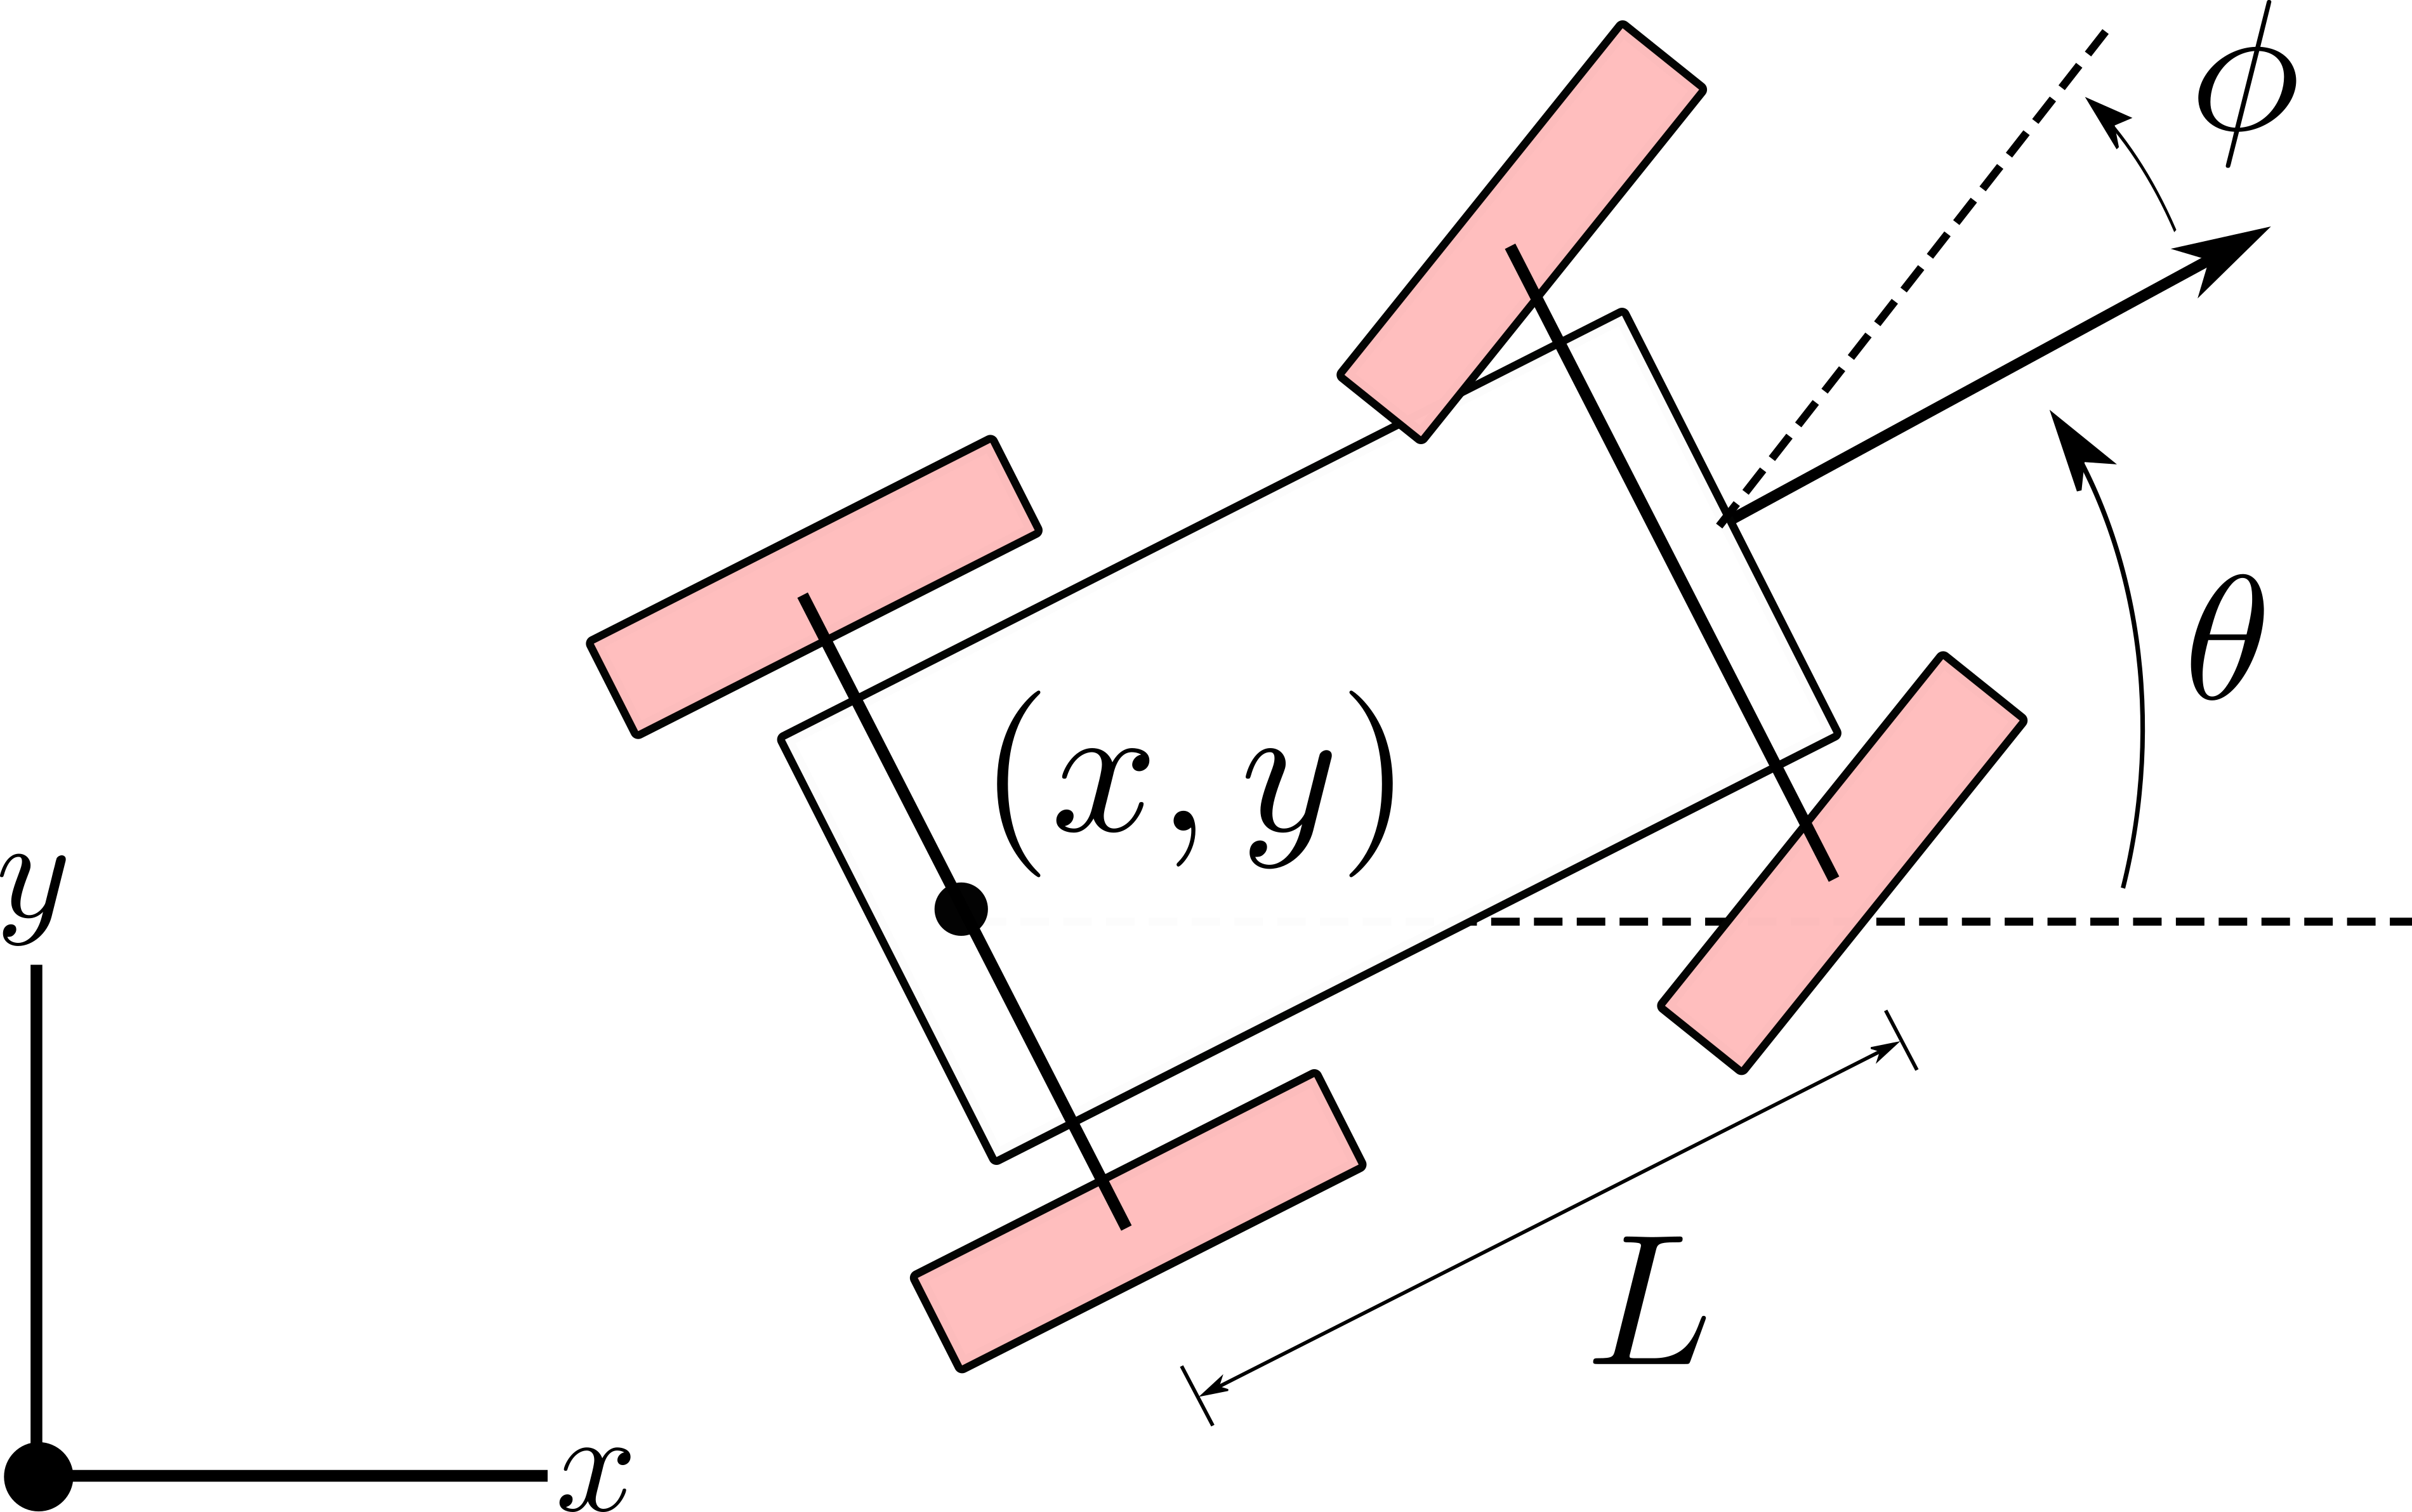
\includegraphics[width=0.95\linewidth]{tex/figs/ch03_figs/car.png}
    \caption{Simple model for an automobile. The state consists of the $(x,y)$ position of the center of the rear axle and the heading angle $\theta$. The control inputs are the steering angle $\phi$ and the forward velocity.}
    \label{fig:car-model} 
\end{marginfigure} 
Consider the car model corresponding to Figure \ref{fig:car-model}:
\begin{equation} \label{eq:car-dynamics}
\begin{split}
    \dot{x} &= v\cos\theta,\\
    \dot{y} &= v\sin\theta,\\
    \dot{\theta} &= \frac{v}{L}\tan\phi, 
\end{split}
\end{equation}
where $(x, y)$ is the position and $\theta$ is the orientation of the vehicle, $v$ is the speed, $\phi$ is the steering angle, and $L$ is the length of the wheelbase. The state $\x$ is therefore defined as $\x = [x, \: y, \: \theta]^T$ and the control is defined as $\bm{u} = [v, \:\phi]^T$.

Suppose the motion planning task is to find a control sequence $\bm{u}(t)$ that will take the car from an initial state $\x_0$ to a final desired state $\x_{f}$. One option would be to formulate an optimal control problem with constraints $\x(t_0) = x_0$ and $\x(t_f) = \x_f$. However, it turns out that for this model there is a simpler approach. In fact, for this model it is sufficient to specify a differentiable trajectory for $x(t)$ and $y(t)$, and the remaining state variables and control inputs can be \textit{analytically} determined!

To see why this is, consider a differentiable trajectory for for $x(t)$ and $y(t)$ with derivatives $\dot{x}(t)$ and $\dot{y}(t)$. From the dynamics model \eqref{eq:car-dynamics} it can be seen that the first two equations can be leveraged to compute $\theta(t)$:
\begin{equation*}
\theta = \tan^{-1}(\dot{y}/\dot{x}).
\end{equation*}
Furthermore, once $\theta(t)$ has been computed the speed is defined:
\begin{equation*}
v = \dot{x}/\cos\theta, \quad \text{or}  \quad v = \dot{y}/\sin\theta.
\end{equation*}
Finally, given $\theta(t)$ and $v(t)$ it is possible to directly solve for the steering angle:
\begin{equation*}
\phi = \tan ^{-1}(\frac{L\dot{\theta}}{v}).
\end{equation*}

This property, that from the specification of a few variables and their derivatives the remaining state and control values are defined, is known as \textit{differential flatness}. 
\end{example}

\begin{definition}[Differential Flatness]
A non-linear system
\begin{equation} \label{eq:diffflatsys}
\dot{\x}(t) = a(\x(t),\bm{u}(t)),
\end{equation}
is differentially flat with flat output $\z$ if there exists a function $\alpha$ such that
\begin{equation}
\z = \alpha (\x,\bm{u},\dot{\bm{u}},\dots,\bm{u}^{(p)}),
\end{equation}
and such that the solutions to the system $\x(t)$ and $\bm{u}(t)$ can be written as functions of the flat output $\z$ and a finite number of its derivatives:
\begin{equation} \label{eq:ztoxu}
\begin{split}
\x &= \beta (\z,\dot{\z},\dots,\z^{(q)}) \\
\bm{u} &= \gamma (\z,\dot{\z},\dots,\z^{(q)}).
\end{split}
\end{equation}
\end{definition}

For a differentially flat system, all of the feasible trajectories for the system can be written as functions of a flat output $\z(t)$ and its time derivatives. Additionally, note that the number of flat outputs is always equal to the number of system inputs. In the context of motion planning and control this is extremely useful for trajectory design because the flat outputs can be specified and then \textit{directly mapped} to the corresponding control inputs.

\subsubsection{Trajectory Design for Differentially Flat Systems}
As previously mentioned, trajectory design for differentially flat systems only requires specification of the trajectories of the flat outputs, which greatly simplifies motion planning and control.

Consider a nonlinear system model of the form \eqref{eq:diffflatsys} that is differentially flat with flat output $\z$ where the objective is to design a trajectory from $\x_0$ to $\x_f$ over a horizon of $T$ seconds. First, find the boundary conditions for the flat output $\z(0)$ and $\z(T)$ that satisfy the boundary conditions on $\x$ by noting that
\begin{equation} \label{eq:flatbc}
\begin{split}
\x_0 &= \beta (\z(0),\dot{\z}(0),\dots,\z^{(q)}(0)), \\
\x_f &= \beta (\z(T),\dot{\z}(T),\dots,\z^{(q)}(T)). \\
\end{split}
\end{equation}
Second, compute \textit{any} smooth trajectory for the flat outputs $\z(t)$ that satisfy these boundary conditions. Third, use \eqref{eq:ztoxu} to map the flat output trajectory $\z(t)$ to the state and control trajectories $\x(t)$ and $\bm{u}(t)$.

Since the flat outputs can be specified as any smooth trajectory, a common choice is to parameterize them using $N$ smooth basis functions:
\begin{equation} \label{eq:flat}
z_j(t) = \sum_{i=1}^{N} \alpha_i^{[j]} \psi_i(t),
\end{equation}
where $z_j$ is the $j$-th element of $\z$, $\alpha_i^{[j]} \in \mathbb{R}$ are variables that parameterize the trajectory and $\psi_i(t)$ are the smooth basis functions. One potential choice is to use polynomial basis functions $\psi_1(t) = 1$, $\psi_2(t) = t$, $\psi_3(t) = t^2$, and so on. Another advantage of choosing this parameterization of $z_j(t)$ is that it is linear in the variables $\alpha_i^{[j]}$. This makes it easy to map specifications on $\z$ into values for $\alpha_i$ that define the trajectory. Consider differentiating \eqref{eq:flat} $q$ times:
\begin{equation}
\begin{split}
\dot{z}_j(t) &= \sum_{i=1}^{N} \alpha_i^{[j]} \dot{\psi_i}(t), \\
&\vdots \\
z_j^{(q)}(t) &= \sum_{i=1}^{N} \alpha_i^{[j]} \psi_i^{(q)}(t). \\
\end{split}
\end{equation}
Now, from the initial and final conditions $z_j(0), \: \dot{z}_j(0), \: \dots , z_j^{(q)}(0)$ and $z_j(T), \: \dot{z}_j(T), \: \dots , z_j^{(q)}(T)$ the coefficients $\alpha_i^{[j]}$ can be computed by solving the following linear system (assuming the matrix is full rank):
\begin{equation} \label{eq:diffflatlinear}
\begin{bmatrix}
    \psi_1(0) & \psi_2(0) & \dots & \psi_N(0) \\
    \dot{\psi_1}(0) & \dot{\psi_2}(0) & \dots & \dot{\psi_N}(0) \\
    \vdots & \vdots & & \vdots \\
    \psi_1^{(q)}(0) & \psi_2^{(q)}(0) & \dots & \psi_N^{(q)}(0) \\
    \psi_1(T) & \psi_2(T) & \dots & \psi_N(T) \\
    \dot{\psi_1}(T) & \dot{\psi_2}(T) & \dots & \dot{\psi_N}(T) \\
    \vdots & \vdots & & \vdots \\
    \psi_1^{(q)}(T) & \psi_2^{(q)}(T) & \dots & \psi_N^{(q)}(T) \\
\end{bmatrix}
\begin{bmatrix}
    \alpha_1^{[j]} \\
    \alpha_2^{[j]} \\
    \vdots \\
    \alpha_N^{[j]} \\
\end{bmatrix} =
\begin{bmatrix}
    z_j(0) \\
    \dot{z}_j(0) \\
    \vdots \\
    z^{(q)}_j(0) \\
    z_j(T) \\
    \dot{z}_j(T) \\
    \vdots \\
    z_j^{(q)}(T)
\end{bmatrix}.
\end{equation}
Once the values for $\alpha_i^{[j]}$ are known, the entire trajectory $z_j(t)$ is therefore known!

Note that this approach is not strictly limited to specifying the initial and final conditions. It is also possible to specify other constraints on $z_j$ and its derivatives as long as they are \textit{equality} constraints. This is accomplished by simply adding equations corresponding to the desired constraints to the linear system of equations \eqref{eq:diffflatlinear}. However, if too many constraints are added the linear system \eqref{eq:diffflatlinear} may not have a solution (i.e. the system is over-determined). Assuming the constraints are not conflicting, this problem can typically be fixed by adding additional basis functions.

To summarize, for differentially flat nonlinear systems, the motion planning and control problem can be greatly simplified by planning in the flat output space. This is possible because of nonlinear functions that allow the flat output trajectory to be directly mapped to state and control trajectories that satisfy the system dynamics.


\subsubsection{Constraints and Time Scaling}
As previously shown, some constraints (e.g. boundary conditions) can be imposed on the trajectory by converting them into conditions on $\z$ and its derivatives, and then solving the linear system of equations \eqref{eq:diffflatlinear}. However, applying \textit{bound} constraints can be slightly more challenging since they are expressed as inequality constraints rather than equality constraints. Nonetheless, bound constraints are common in robotics and therefore it is important to be able to consider them in the trajectory generation process. For example, the simple car robot from Example \ref{ex:carflatness} could have an upper bound on its speed: 
\begin{equation*}
|v(t)| \leq v_\text{max}.
\end{equation*}

One technique for handling these types of constraints is to use \textit{time scaling}. The general approach to satisfy bound constraints by time scaling is:
\begin{enumerate}
    \item Specify boundary conditions and solve the linear system of equations \eqref{eq:diffflatlinear} to get a candidate trajectory $\x(t)$ with control inputs $\bm{u}(t)$.
    \item If the candidate trajectory violates any bound constraints, generate a new trajectory by keeping the same geometric \textit{path} but decreasing the rate at which it moves along the path.
\end{enumerate}

\subsubsection{Geometric Path}
A geometric path is a sequence of states for the robot that is not associated with time. Given a candidate trajectory $\x(t)$, the geometric path can be defined by alternatively expressing the trajectory as $\x(t) = \x(s(t))$ where $s$ is a new ``path'' parameter and $s(t)$ is defined with $s(0) = s_0$, $s(T) = s_f$, and $\dot{s}(t) > 0$. A common choice for the path parameter $s$ is the arc length along the path. The geometric trajectory is then written as just $\x(s)$, such that the state is now a function of the position along the path and not time. Note that $\x(t): [0,T] \xrightarrow{} \R^n$ and $\x(s): [s_0, s_f] \xrightarrow{} \R^n$ are actually two different functions. In particular, the function $\x(t)$ can be derived from $\x(s)$ by the definition of the function $s(t): [0,T] \xrightarrow{} [s_0, s_f]$ and the composition $\x(s(t))$.

\subsubsection{Time Scaling}
For some systems, once the geometric path $\x(s)$ has been extracted from the candidate trajectory $\x(t)$, it is possible to arbitrarily redefine new trajectories with different time scales by simply redefining $s(t)$. In other words parts of the original candidate trajectory can be sped up or slowed down as desired. 

To motivate why time scaling is important we can consider a simplified problem that does not involve a dynamics model. In particular, consider a scalar variable $x \in \R$ and a desired geometric path that connects $x_0$ and $x_f$ that is parameterized as $x(s) = x_0 + s(x_f - x_0)$ for $s \in [0,1]$ (note that $x(0) = x_0$ and $x(1) = x_f$). By choosing how $s$ varies in time (i.e. the function $s(t)$) this geometric path can be transformed into many different \textit{trajectories}, $x(t)$. As a simple choice, the function $s(t)$ can be parameterized as the cubic polynomial:
\begin{equation*}
    s(t) = \frac{3}{T^2}t^2 - \frac{2}{T^3}t^3.
\end{equation*}
This specific choice ensures that $s(0) = 0$, $s(T) = 1$, and $\dot{s}(0) = \dot{s}(T) = 0$ such that the trajectory will be defined over the time interval $t \in [0,T]$. Substituting this function into $x(s)$ then yields an expression for the trajectory $x(t)$:
\begin{equation*}
    x(t) = x_0 + \big(\frac{3}{T^2}t^2 - \frac{2}{T^3}t^3 \big)(x_f - x_0).
\end{equation*}
One easy way to scale the trajectory in this case is to simply change $T$, with larger values of $T$ meaning that it will take longer for $x$ to traverse the geometric path from $x_0$ to $x_f$. In fact, the maximum velocity can also be computed as:
\begin{equation*}
    \dot{x}_{\text{max}} = \frac{3}{2T}(x_f - x_0).
\end{equation*}
Therefore, not only does rescaling the trajectory by changing $T$ make the path traversal time change, but it can also be used to decrease quantities such as the maximum velocity!

\paragraph{Time Scaling with Differential Models:}
Some additional considerations need to be made when time-scaling trajectories that must also satisfy differential models.
First, note that the time derivative of the state can be rewritten by using the chain rule:
\begin{equation*}
\dot{\x}(t) = \frac{d\x(t)}{dt} = \frac{d\x(s)}{ds} \frac{ds(t)}{dt}.
\end{equation*}
Now consider a candidate trajectory $\x(t)$ and an associated geometric path $\x(s)$ for some $s(t)$ that is defined over the interval $t\in[0,T]$ with $s(0) = s_0$ and $s(T) = s_f$. Since $\x(t)$ is a trajectory of the dynamics \eqref{eq:diffflatsys}, the geometric path $\x(s)$ and time scaling law $s(t)$ satisfy
\begin{equation}
\frac{d\x(s)}{ds} \frac{ds(t)}{dt} = a(\x(s), \bm{u}(s)),
\end{equation}
for every point $s \in [s_0, s_f]$.

To design a new time scaling law $\tilde{s}(t)$ over some potentially new time interval $t \in [0,\tilde{T}]$ where $\tilde{s}(0) = s_0$ and $\tilde{s}(\tilde{T}) = s_f$, it is important to note that the dynamics equations must still be satisfied\footnote{The geometric path is still defined on the interval $[s_0, s_f]$ so this interval must remain the same for any new time scaling law, but the time interval can change.}. In other words, for every $\tilde{s} \in [s_0, s_f]$:
\begin{equation} \label{eq:stildedynamics}
\frac{d\x(\tilde{s})}{d\tilde{s}} \dot{\tilde{s}} = a(\x(\tilde{s}), \tilde{\bm{u}}(\tilde{s})).
\end{equation}
Since the geometric path is fixed, the terms $\frac{d\x(\tilde{s})}{d\tilde{s}}$ and $\x(\tilde{s})$ are fixed. Thus a new time scaling law $\tilde{s}(t)$ is only admissible if a new control $\tilde{\bm{u}}(\tilde{s})$ can also be found that guarantees that \eqref{eq:stildedynamics} holds.
Luckily, for some specific systems this is easy with the appropriate choice of path parameter $s$.

\begin{example}[Time Scaling for Simple Car Model]
\theoremstyle{definition} Consider again the simple car model \eqref{eq:car-dynamics} from Example \ref{ex:carflatness}. Suppose a candidate trajectory $\x_c(t)$ with control $\bm{u}_c(t)$ has been defined by leveraging the differential flatness of the model (i.e. setting up and solving \eqref{eq:diffflatlinear} and then mapping the flat outputs $\z_c(t)$ into the state and control). For this system a good choice for the path parameter is the arc-length, such that
\begin{equation*}
    s(t) = \int_0^t v(t') dt', \quad \dot{s}(t) = v(t).
\end{equation*}

With this choice of path parameter the geometric path function $\x_c(s)$, $s_0 = 0$, and $s_f = L_{\text{path}}$ are all fixed (where $L_{\text{path}}$ is the total length of the path). Rewriting the dynamics \eqref{eq:stildedynamics} based on the simple car model:
\begin{equation*}
\begin{split}
\frac{dx_c(\tilde{s})}{d\tilde{s}}\dot{\tilde{s}} &= v(\tilde{s})\cos\theta_c(\tilde{s}),\\
\frac{dy_c(\tilde{s})}{d\tilde{s}}\dot{\tilde{s}}&= v(\tilde{s})\sin\theta_c(\tilde{s}),\\
\frac{d\theta_c(\tilde{s})}{d\tilde{s}}\dot{\tilde{s}} &= \frac{v(\tilde{s})}{L}\tan\phi(\tilde{s}).
\end{split}
\end{equation*}
Any choice of the time scaling function $\tilde{s}(t)$ must be able to satisfy these equations, and note that the trivial choice of $\tilde{s}(t) = s(t)$ will automatically satisfy these equations with the candidate control inputs $\bm{u}_c(t)$. 

Since the choice of the path parameter yields $\dot{\tilde{s}} = v(\tilde{s})$, these equations can be further simplified:
\begin{equation*}
\begin{split}
\frac{dx_c(\tilde{s})}{d\tilde{s}} &= \cos\theta_c(\tilde{s}),\\
\frac{dy_c(\tilde{s})}{d\tilde{s}}&= \sin\theta_c(\tilde{s}),\\
\frac{d\theta_c(\tilde{s})}{d\tilde{s}} &= \frac{1}{L}\tan\phi(\tilde{s}).
\end{split}
\end{equation*}
The first two equations are guaranteed to be satisfied for all $\tilde{s} \in [s_0, s_f]$ because the original candidate trajectory satisfies the dynamics. Additionally, the third equation is guaranteed to be satisfied by choosing $\phi(\tilde{s}) = \phi_c(\tilde{s})$ (i.e. using the same steering input as with the candidate trajectory).

This is interesting because it means that the equations are all satisfied \textit{independently} of the choice of $\dot{\tilde{s}}$. Therefore, since $\dot{\tilde{s}} = v(\tilde{s})$ this means that the speed input can be chosen arbitrarily while maintaining the same geometric path! This is extremely useful because it means that bound constraints on the speed $\lvert v(t)\rvert \leq v_\text{max}$ can be easily enforced.
\end{example}


\paragraph{Time Scaling with Kinematic Models:} Time-scaling trajectories is much more straightforward when kinematic models are used. Consider the case where the model of the system is derived from $k$ Pfaffian constraints $\bm{A}^T(\x)\dot{\x} = 0$. In this case the kinematic model can be written in the form:
\begin{equation} \label{eq:kinmodel}
    \dot{\x} = G(\x) \bu,
\end{equation}
where the columns of the matrix $G(\x)$ span the null space of the matrix $A^T(\x)$. Now again consider a path parameter $s$ that is used to reparameterize trajectories $\x(t)$ as $\x(s(t))$, and satisfies $s(0) = s_0$, $s(T) = s_f$, and $\dot{s}(t) > 0$\footnote{The condition $\dot{s}(t) > 0$ is critical to ensure that the function $s(t)$ is invertible. In other words, to guarantee that there is a one-to-one mapping between $t$ and $s$.}. Rewriting the time derivative of the state using the chain rule yields:
\begin{equation}
    \frac{d\x(s)}{ds} \dot{s} = G(\x) \bu(t).
\end{equation}
By making a substitution that $\bu(t) =  \bu_g(s)\dot{s}$ the dynamics can be further written as:
\begin{equation} \label{eq:kinematicgeometricmodel}
    \frac{d\x(s)}{ds} = G(\x)\bu_g(s).
\end{equation}
The terms $\bu_g(s)$ are referred to as \textit{geometric controls}, since they are defined only with respect to the path parameter $s$. Critically, \eqref{eq:kinematicgeometricmodel} says that once the geometric controls $\bu_g(s)$ are defined, the entire geometric path $\x(s)$ is also defined! The choice of the timing law $s(t)$ can then be chosen in any manner and it will not change the geometric path, but will change the time trajectory $\x(t)$. In particular, once the geometric control $\bu_g(s)$ and timing law are chosen, the actual controls are computed simply by the previous relationship $\bu(t) =  \bu_g(s)\dot{s}$.

Based on this analysis, the procedure for \textit{rescaling} a trajectory of a kinematic model can be made more concrete. First, consider a given trajectory $\x(t)$ with control $\bu(t)$ defined over $t \in [0,T]$ that satisfies the kinematic model \eqref{eq:kinmodel}. For simplicity, consider the path parameter $s$ to be arc-length of the trajectory such that $s(0) = 0$ and $s(T) = L_{\text{path}}$.
The following steps can then be used to define a new control input $\tilde{\bu}(t)$ that will make the kinematic model follow the same geometric path but with a different time scale:
\begin{enumerate}
\item Determine $s(t)$ based on the original trajectory $\x(t)$. In other words, figure out how far along the trajectory the system is at each time $t$. Then reparameterize the control $\bu(t)$ as a function of $s$, $\bu(s(t))$. 
\item Compute the geometric controls $\bu_g(s) = \bu(s(t))/\dot{s}(t)$ for each point $s \in [s_0, s_f]$.
\item Define a new timing law $\tilde{s}(t)$ that satisfies $\tilde{s}(0) = 0$ and $\tilde{s}(\tilde{T}) = L_{\text{path}}$ with $\dot{\tilde{s}} > 0$ over the interval $[0, \tilde{T}]$.
\item Compute the new control $\tilde{\bu}(t) = \bu_g(\tilde{s}(t)) \dot{\tilde{s}}(t)$ for all $t \in [0, \tilde{T}]$.
\end{enumerate}


\begin{example}[Time Scaling for Unicycle Model] \label{ex:timescaleuni}
\theoremstyle{definition}
Consider the kinematic unicycle model:
\begin{equation} \label{eq:unicycle}
\begin{split}
    \dot{x} &= v\cos\theta,\\
    \dot{y} &= v\sin\theta,\\
    \dot{\theta} &= \omega, 
\end{split}
\end{equation}
where $(x, y)$ is the position and $\theta$ is the orientation, $v$ is the speed, and $\omega$ is the rotation rate. The state $\x$ is defined as $\x = [x, \: y, \: \theta]^T$ and the control is defined as $\bm{u} = [v, \:\omega]^T$.

To time-scale trajectories of this system, consider the use of arc-length as path parameter:
\begin{equation*}
    s(t) = \int_0^t v(\tau) d\tau, \quad \dot{s}(t) = v(t),
\end{equation*}
such that for a trajectory defined on the interval $t \in [0,T]$ with total length $L_{\text{path}}$, the path parameter is defined with $s(0) = 0$ and $s(T) = L_{\text{path}}$.
With this choice, the geometric controls are given by:
\begin{equation*}
\begin{split}
v_g(s) &= \frac{v(s)}{\dot{s}(t)} = 1, \\
\omega_g(s) &= \frac{\omega(s)}{\dot{s}(t)} = \frac{\omega(s)}{v(s)},
\end{split}
\end{equation*}
where $v(s(t))$ has been substituted in for $\dot{s}(t)$.
Therefore if a new timing law $\tilde{s}(t)$ is introduced this will automatically define a new velocity $\tilde{v}(\tilde{s})$ at each point $\tilde{s}$, which can then be used to solve for the new $\tilde{\omega}$ inputs by:
\begin{equation*}
\begin{split}
\tilde{\omega}(\tilde{s}) &= \omega_g(\tilde{s}) \dot{\tilde{s}}(t) = \frac{\omega(\tilde{s})}{v(\tilde{s})} \tilde{v}(\tilde{s}).
\end{split}
\end{equation*}
Alternatively, since it is easier to work with the velocity directly rather than $\tilde{s}(t)$, in this case it is possible to just specify $\tilde{v}(\tilde{s})$ for all $\tilde{s} \in [0, L_{\text{path}}]$ and then to compute $\tilde{\omega}(\tilde{s}) = \frac{\omega(\tilde{s})}{v(\tilde{s})} \tilde{v}(\tilde{s})$. Then, to determine the new controls as functions of time rather than $\tilde{s}$, it can be noted that
\begin{equation*}
    \tau(s) = \int_0^s \frac{ds'}{\tilde{v}(s')},
\end{equation*}
defines a function $\tau(s)$ that maps each point $s \in [0, L_{\text{path}}]$ to a new time.
\end{example}


\subsection{Exercises}
\subsubsection{Trajectory Generation via Differential Flatness}
Complete \textit{Problem 1:  Trajectory Generation via Differential Flatness} located in the online repository:

\vspace{\baselineskip}

\url{https://github.com/PrinciplesofRobotAutonomy/AA274A_HW1},

\vspace{\baselineskip}

where you will use an extended unicycle model to practice generating dynamically feasible trajectories by levering the system's differential flatness property. You will also have the chance to use time scaling techniques to design trajectories that satisfy control constraints.

 


